\documentclass[a4paper,12pt]{article}

\usepackage{url}
\usepackage{epsfig}
\usepackage{graphics}
\usepackage{fancyhdr}
\usepackage[table,xcdraw]{xcolor}
\usepackage{graphicx}
\usepackage{amsmath}
\usepackage[space]{grffile}
\graphicspath{{pictures/}}

\title{Lyrics Predictor report for the course DD2380}
\author{\hspace*{-0.5cm}
GROUP 9\\
\begin{tabular}{cccc}
Salma El Alaoui & Rongrong Qi & J.Theodoridis & Guisong Fu\\
%931007-T148 & 920831T267 & 900302T459 & 9209173914 \\
salmaeat@kth.se & rqi@kthse & johthe@kth.se & guisong@kth.se \\
\end{tabular}} 
% Normally there will not be any pictures but we want
% these so that we can connect faces to names in the course
% We also want birthdates so that we can tell people with the same
% name apart
\date{}

\pagestyle{fancy}
\setlength{\headheight}{15pt}
\fancyhf{}
\lhead{DD2380 ai15} % DO NOT REMOVE!!!!
\rhead{Salma El Alaoui, Rongrong Qi, Johannes Theo, Guisong Fu} %% UPDATE WITH YOUR NAMES

\begin{document}

\maketitle
\thispagestyle{fancy}




\clearpage

%%%%%%%%%%%%%%%%%%%%%%%%%%%%%%%%%%%%%%%%%%%%%%%%%%%%%%%%%%%%%
%%%%%%%%%%%%%%%%%%%%%%%%%%%%%%%%%%%%%%%%%%%%%%%%%%%%%%%%%%%%%

\section{Introduction}
\label{sec:intro}
Music and lyrics can appear in various forms, therefore the difference between genres is a rich field for experimentation and research. In this paper we evaluate a word predictor for song lyrics by comparing the two musical genres: POP and ROCK. Furthermore we perform some corpus analysis and compare different N-Gram models, smoothing techniques and tagging methods.
%%%%%%%%%%%%%%%%%%%%%%%%%%%%%%%%%%%%%%%%%%%%%%%%%%%%%%%%%%%%%
%%%%%%%%%%%%%%%%%%%%%%%%%%%%%%%%%%%%%%%%%%%%%%%%%%%%%%%%%%%%%
\section{Related work}
\label{sec:relwork}

There has been a lot of research in the field of song lyrics for instance analysis of texts or work of rhyme. Since we decided to place our project in that field, we see the Rap Lyrics Generator from Nguyen and Sa \cite{hieu2009rap} as a starting point for our work. Although have not implemented any rhyming grammar we use some ideas for our corpus building and cleaning implementation.

From personal experience we expect the lyrics to have their own characteristics in each category. In a more sophisticated way this has been subject of research in a paper \cite{smith2012your} where lyrics have been analyzed in the context of stereotypes. As they, we use collocations to find words that appear together frequently. We expect them to be highly different in each category and therefore important when evaluating the results of the word predictors.

According to Manning and Schuetze \cite[p.155]{manning1999foundations} a "COLLOCATION is an expression consisting of two or more words that
correspond to some conventional way of saying things". More technical, collocations are n-grams of limited compositionality. As presented in their book we will use the Pointwise Mutual Information (PMI) measure to rate and rank our collocations.

%%%%%%%%%%%%%%%%%%%%%%%%%%%%%%%%%%%%%%%%%%%%%%%%%%%%%%%%%%%%%
%%%%%%%%%%%%%%%%%%%%%%%%%%%%%%%%%%%%%%%%%%%%%%%%%%%%%%%%%%%%%
\section{Method}
\label{sec:method}
\subsection{Corpus}

To build a lyric corpus we crawled the lyrics website \url{http://www.chartlyrics.com/} using their API. The retrieved lyrics were cleaned and later categorized in an extra category file. Our main corpus is a collection of 1697 lyrics from 59 different artist divided in 2 main categories. To have a big contrast between the categories we selected artists from the genres pop and rock and from all times. This way we have a variety in our corpus that ranges from ABBA to AC/DC as well as from Lady Gaga to Metallica. 

\subsubsection{Corpus Analysis}
To evaluate our corpus we perform some basic measurements such as total amount of words, vocabulary and text richness and compare them to the well known brown corpus. Furthermore we compare the top 5 collocations for each category using bi- and trigrams. This way we can verify the quality of the corpus as baseline for our later experiments 

\subsection{Word predictor}
\subsubsection{Simple N-Gram model}
The intuition of the N-gram model is that instead of computing the probability of a word given its entire history, we will approximate the history by just the last few words. That assumption is a Markov assumption, Markov models being probabilistic models that assume that we can predict the probability of some future unit without looking too far in the past. \\
The general equation for the N-gram approximation to the conditional probability of the next word in a sequence is:
\begin{equation}
P(w_n|w_1^{n-1}) \approx P(w_n|w_{n-1}^{n-N+1})
\end{equation}
In the simple N-gram model, we estimate these probabilities using the Maximum likelihood estimate, by taking counts from the corpus and normalizing them.
\begin{equation}
P(w_n|w_{n-1}^{n-N+1}) = \frac{C(w_{n-1}^{n-N+1} w_{n})}{C(w_{n-1}^{n-N+1})}
\end{equation}
\subsubsection{Smoothing}
The problem with the maximum likelihood estimation process for training the parameters of the simple N-gram model is sparse data. That is caused by the fact that our maximum likelihood estimate was based on a particular instance of training data: because the training corpus is limited, some perfectly correct English word sequences will be missing from it. The MLE estimate also produces poor estimates when the counts are non-zero but still small.
For these reasons, we will modify the maximum likelihood estimate for computing N-gram probabilities, focusing on the N-gram events to which we incorrectly assigned zero probability because they have zero frequency counts.
\paragraph{Laplace Smoothing}
One simple way to do smoothing is to take the matrix of N-gram counts before they are normalized into probabilities and add one to all the counts. 
For Laplace smoothed bigram counts for example, the probability becomes: 
\begin{equation}
P_{Laplace}(w_n|w_{n_1}) = \frac{C(w_n w_{n_1})}{C(w_{n-1}) + V}
\end{equation}
$V$ is the number of words in the vocabulary. Since each one got incremented, we also need to adjust the denominator to take into account the extra V observations.
\subsubsection{Back-off}
While smoothing can help solve the problem of zero frequency N-grams, there is an additional source of information we can use: 
If we are trying to compute the probability of a particular N-gram, but have no examples of it in the corpus, we can estimate its probability by using a lower degree N-gram.\\
In the Katz backoff N-gram model, if the N-gram we need has zero counts, we approximate it by backing off to the N-1 gram. We continue backing off until we reach a history that has some counts.
\[
P_{katz}(w_n|w_{n-N+1}^{n-1}) =
\begin{cases}
    P(w_n|w_{n_N+1}^{n-1}), & \text{if } C(w_{n-N+1}^{n})> 0\\
    \alpha(w_{n_N+1}^{n-1}\times P_{katz}(w_n|w_{n-N+2}^{n-1}),  & \text{otherwise.}
\end{cases}
\]
The backoff weight $\alpha$ passes the left-over probability mass to the lower order N-grams.
For a given (N-1)-gram context, the total left-over probability mass can be computed by subtracting from the total probability mass for all N-grams starting with that context. This gives ud the total probability mass that we are ready to distribute to all (N-1)-grams. We then need to normalize it by the total probability of all the (N-1)-grams that begin some N-gram which has zero counts. Thus $\alpha$ is a function of the preceding word.\\

\subsubsection{N-Gram Tagging}
A part-of-speech tagger, or POS-tagger, processes a sequence of words, and attaches a part of speech tag to each word.\cite{NLTK} N-Gram tagging is similar to N-Gram model. Instead of computing the probability of a word by the history of few words before it, we will compute the probability of the tag of a word, by the history of this word and the tag history of few words before it.
\begin{equation}
P(t_n|w_n,t_{n-1}^{n-N+1}) = \frac{C(t_{n-1}^{n-N+1} w_{n},t_{n})}{C(t_{n-1}^{n-N+1}w_{n})}
\end{equation}

\subsubsection{Linear combination}
The Linear Combination algorithm \cite{tagging} combines an N-gram tagger and N-gram word model. The final probability is a weighted combination of the two models. If we take the example of a tag trigram and a word bigram, the probability becomes:
\begin{equation}
P(w_i|w_{i-1},t_{i-1},t_{i-2}) 
=\alpha \times P(w_{i}|w_{i-1})+(1 - \alpha) \times \max_{t_i \in T(w_i)}[P(w_i|t_i) \times P(t_i|t_{i-1},t_{i-2})]
\end{equation}
As we can see from the equation, in the first model, we attempt to find the most likely tag for the current position according
to the two previous part-of-speech tags, and then
look for words that have the highest probability of
being in the current position given the most likely
tag for this position and the previous word. The second model is the simple bigram model. \\
$\alpha$ is the coefficient of the linear combination that weights both factors. $\alpha$ is determined experimentally.
 
\subsection{Implementation}

We implemented the whole project in python 3.4 using nltk 3. Figure~\ref{fig:workflow} shows our basic workflow from building the corpus to the analysis and prediction.

\begin{figure}
\centering
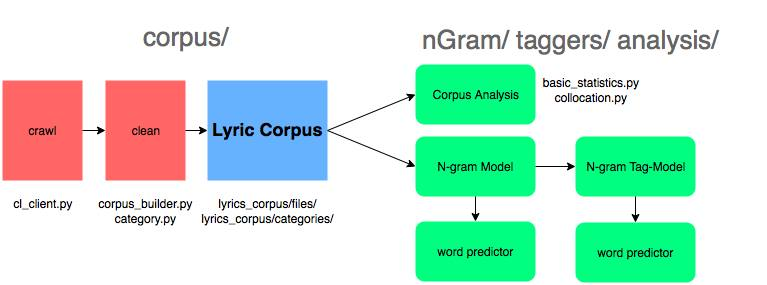
\includegraphics[width=1\linewidth]{workflow}
\caption{Worklow for building the lyric corpus and performing experiments.}
\label{fig:workflow}
\end{figure}



%%%%%%%%%%%%%%%%%%%%%%%%%%%%%%%%%%%%%%%%%%%%%%%%%%%%%%%%%%%%%
%%%%%%%%%%%%%%%%%%%%%%%%%%%%%%%%%%%%%%%%%%%%%%%%%%%%%%%%%%%%%
\section{Experimental results}

\subsection{Experiments}

\subsubsection{Basic Statistics}

\begin{figure}[!htb]
\centering
\minipage{0.47\textwidth}
  \centering
  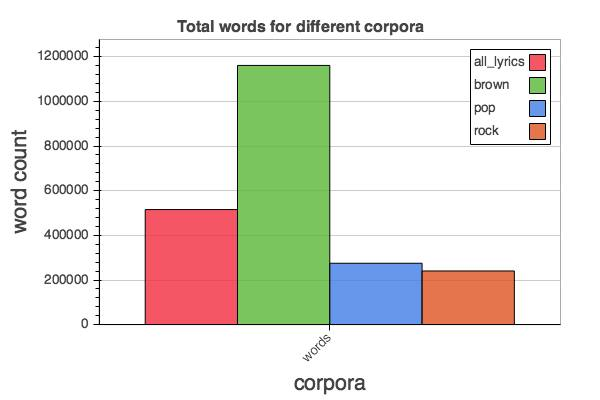
\includegraphics[width=1\linewidth]{word}
  \caption{The total amount of words per corpus.}\label{fig:words}
\endminipage\hfill
\minipage{0.47\textwidth}
  \centering
  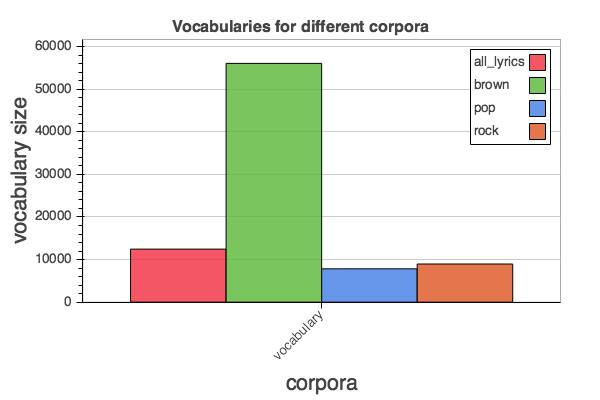
\includegraphics[width=1\linewidth]{vocab}
  \caption{Size of the vocabularies.}\label{fig:vocabulary}
\endminipage\hfill
\end{figure}

\begin{figure}
\centering
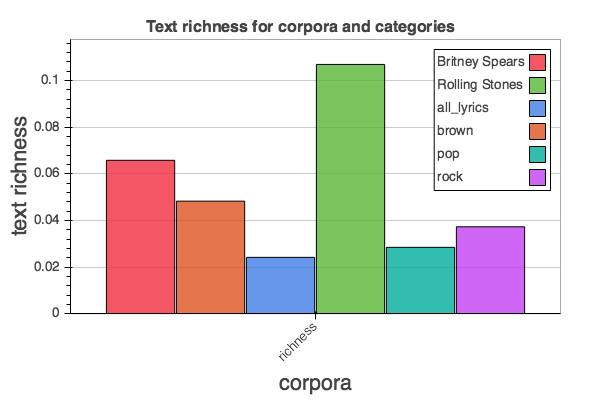
\includegraphics[width=0.5\linewidth]{richness}
\caption{The text richness for different corpora and artists. Text richness in this context is defined as total amount of words divided by the size of vocabulary.}
\label{fig:richness}
\end{figure}


From figure~\ref{fig:words} we can observe that our corpus has a total of 515477 words which is about 44 percent of the brown corpus size provided by the nltk package. More important for our further work is the fact, that the word count for the categories ROCK (240448) and POP (275029) is almost equally distributed. Figure~\ref{fig:vocabulary} shows that the brown corpus has a vocabulary of 56057 words. This is almost 4.5 times more compared to our corpus which has only 12460 different words but the two categories are again almost equally distributed.
Text richness as shown in figure~\ref{fig:richness}, indicates a similar distribution for the categories. Note that the score can vary vastly from average for specific artists.

\subsubsection{Collocations}
We extract bi- and trigram collocations for the POP and ROCK categories. According to Manning and Schuetze \cite{manning1999foundations} we use the PMI measure to calculate and rank our collocations. In addition we print the frequency distribution. The search window was 2 for bigrams and 3 for trigrams. To eliminate extremely rare collocations we applied a minimum frequency filter of 10 for bigrams and 5 for trigrams. Table~\ref{tab:top_collocation} shows the top 5 results for each combination of our experiment. Note the relatively high score for the trigram collocations. 

\begin{table}[]
\centering
\label{tab:top_collocation}
\begin{tabular}{|l|l|l|l|l|l|l|}
\hline
\rowcolor[HTML]{C0C0C0} 
\multicolumn{3}{|c|}{\cellcolor[HTML]{C0C0C0}{\color[HTML]{000000} \textbf{POP}}} & {\color[HTML]{000000} } & \multicolumn{3}{c|}{\cellcolor[HTML]{C0C0C0}{\color[HTML]{000000} \textbf{ROCK}}} \\ \hline
\rowcolor[HTML]{C0C0C0} 
\textbf{collocation}           & \textbf{pmi}      & \textbf{fDist}     &                         & \textbf{collocation}        & \textbf{pmi}       & \textbf{fDist}       \\ \hline
kitty kat                      & 14.26                   & 14                     &                         & arnold layne                & 14.41                    & 11                       \\ \hline
raspberry beret                & 14.26                   & 12                     &                         & killboy powerhead           & 14.29                    & 12                       \\ \hline
mamma mia                      & 14.16                   & 10                     &                         & mi corazn                   & 14.29                    & 12                       \\ \hline
tick tock                      & 13.98                   & 14                     &                         & organic anti                & 14.17                    & 10                       \\ \hline
sugar coated                   & 13.31                   & 10                     &                         & 53rd 3rd                    & 14.17                    & 13                       \\ \hline
\rowcolor[HTML]{EFEFEF} 
coucher avec moi               & 30.13                   & 8                      &                         & franco un american          & 29.62                    & 5                        \\ \hline
\rowcolor[HTML]{EFEFEF} 
christopher tracys parade      & 29.13                   & 7                      &                         & dub thee unforgiven         & 29.05                    & 8                        \\ \hline
\rowcolor[HTML]{EFEFEF} 
vous coucher avec              & 28.28                   & 8                      &                         & yak yak yak                 & 28.56                    & 5                        \\ \hline
\rowcolor[HTML]{EFEFEF} 
jumping thumping shout         & 27.68                   & 6                      &                         & twentieth century fox       & 28.46                    & 9                        \\ \hline
\rowcolor[HTML]{EFEFEF} 
creole lady marmalade          & 27.38                   & 5                      &                         & longer shop happily         & 27.75                    & 9                        \\ \hline
\end{tabular}
\caption{Top 5 bi- and trigram collocations ranked by pmi score.}
\end{table}



\subsubsection{Random sentence generation}
We generate random sentences from bigram, trigram and quadrigram models trained on our song corpus. Table~\ref{tab:randomSents} shows the results.

\begin{table}[]
\centering
\resizebox{\textwidth}{!}{%
\begin{tabular}{|l|l|}
\hline
\rowcolor[HTML]{EFEFEF} 
\textbf{Ngrams} & \multicolumn{1}{c|}{\cellcolor[HTML]{EFEFEF}\textbf{Sentences}} \\ \hline
\textbf{Bigram} & still. i am a little girl. \\ \hline
\textbf{} & leaves are the way. i am a little girl \\ \hline
\textbf{} & aaaaaa. i am a little girl \\ \hline
\textbf{Trigram} & awoke my sense. you are the one. \\ \hline
\textbf{} & another was born to make you feel it. \\ \hline
\textbf{} & shes juicy and shes got the jack. \\ \hline
\textbf{Quadrigram} & my memory races at speeds. come on. come on. \\ \hline
\textbf{} & everything crumbles sooner or later. you are the one i am dreaming of. \\ \hline
\textbf{} & on dancing shadows from behind. but now i have got to give. \\ \hline
\end{tabular}
}
\caption{Sentences generated from N-gram models randomly}
\label{tab:randomSents}
\end{table}
The longer the context on which we train the model, the more coherent the sentences.The bigram sentences have some very local word-to-word
coherence (especially if we consider that punctuation counts as a word). The trigram and quadrigram sentences are beginning to look a lot like song lyrics.

\subsubsection{Bigram counts and probabilities}
In order to test the correctness of smoothing methods, we choose sentence ``and i do not wanna miss a thing" to compute bigram counts without smoothing(simple Ngram), showed in Table~\ref{tab:countsNgram}. And then compute bigram probability with Laplace and Witten Bell smoothing methods. The results are in Table~\ref{tab:probLaplace} and Table~\ref{tab:probWittenBell} separately.
\begin{table}[]
\centering
\begin{tabular}{|
>{\columncolor[HTML]{EFEFEF}}c |c|c|c|c|c|c|c|c|}
\hline
               & \cellcolor[HTML]{EFEFEF}\textbf{and} & \cellcolor[HTML]{EFEFEF}\textbf{i} & \cellcolor[HTML]{EFEFEF}\textbf{do} & \cellcolor[HTML]{EFEFEF}\textbf{not} & \cellcolor[HTML]{EFEFEF}\textbf{wanna} & \cellcolor[HTML]{EFEFEF}\textbf{miss} & \cellcolor[HTML]{EFEFEF}\textbf{a} & \cellcolor[HTML]{EFEFEF}\textbf{thing} \\ \hline
\textbf{and}   & 0                                    & 1288                               & 75                                  & 23                                   & 0                                      & 0                                     & 133                                & 0                                      \\ \hline
\textbf{i}     & 5                                    & 68                                 & 892                                 & 1                                    & 348                                    & 59                                    & 0                                  & 0                                      \\ \hline
\textbf{do}    & 2                                    & 81                                 & 119                                 & 2656                                 & 0                                      & 0                                     & 12                                 & 0                                      \\ \hline
\textbf{not}   & 2                                    & 21                                 & 60                                  & 0                                    & 138                                    & 5                                     & 91                                 & 0                                      \\ \hline
\textbf{wanna} & 0                                    & 0                                  & 39                                  & 0                                    & 0                                      & 4                                     & 0                                  & 0                                      \\ \hline
\textbf{miss}  & 0                                    & 0                                  & 0                                   & 0                                    & 0                                      & 0                                     & 0                                  & 0                                      \\ \hline
\textbf{a}     & 0                                    & 22                                 & 4                                   & 0                                    & 1                                      & 0                                     & 23                                 & 47                                     \\ \hline
\textbf{thing} & 0                                    & 37                                 & 0                                   & 0                                    & 0                                      & 0                                     & 0                                  & 0                                      \\ \hline

\end{tabular}
\caption{Bigram counts for simple Ngram}
\label{tab:countsNgram}
\end{table}

\begin{table}[]
\centering
\resizebox{\textwidth}{!}{%
\begin{tabular}{|
>{\columncolor[HTML]{EFEFEF}}c |c|c|c|c|c|c|c|c|}
\hline
 & \cellcolor[HTML]{EFEFEF}\textbf{and} & \cellcolor[HTML]{EFEFEF}\textbf{i} & \cellcolor[HTML]{EFEFEF}\textbf{do} & \cellcolor[HTML]{EFEFEF}\textbf{not} & \cellcolor[HTML]{EFEFEF}\textbf{wanna} & \cellcolor[HTML]{EFEFEF}\textbf{miss} & \cellcolor[HTML]{EFEFEF}\textbf{a} & \cellcolor[HTML]{EFEFEF}\textbf{thing} \\ \hline
\textbf{and} & 9.9E-06 & 0.0128 & 0.0008 & 0.0002 & 9.9E-06 & 9.9E-06 & 0.0013 & 9.9E-06 \\ \hline
\textbf{i} & 5.3E-05 & 0.0006 & 0.0079 & 1.8E-05 & 0.0031 & 0.0005 & 8.9E-06 & 8.9E-06 \\ \hline
\textbf{do} & 3.1E-05 & 0.0008 & 0.0012 & 0.0275 & 1.0E-05 & 1.0E-05 & 0.0001 & 1.0E-05 \\ \hline
\textbf{not} & 3.1E-05 & 0.0002 & 0.0006 & 1.0E-05 & 0.0014 & 6.1E-05 & 0.0009 & 1.0E-05 \\ \hline
\textbf{wanna} & 1.1E-05 & 1.1E-05 & 0.0004 & 1.1E-05 & 1.1E-05 & 5.4E-05 & 1.1E-05 & 1.1E-05 \\ \hline
\textbf{miss} & 1.1E-05 & 1.1E-05 & 1.1E-05 & 1.1E-05 & 1.1E-05 & 1.1E-05 & 5.4E-05 & 1.1E-05 \\ \hline
\textbf{a} & 9.9E-06 & 0.0002 & 4.9E-05 & 9.9E-06 & 2.0E-05 & 9.9E-06 & 0.0002 & 0.0005 \\ \hline
\textbf{thing} & 1.1E-05 & 0.0004 & 1.1E-05 & 1.1E-05 & 1.1E-05 & 1.1E-05 & 1.1E-05 & 1.09E-05 \\ \hline
\end{tabular}
}
\caption{Bigram probability with Laplace Smoothing Ngram}
\label{tab:probLaplace}
\end{table}

\begin{table}[]
\centering
\resizebox{\textwidth}{!}{%
\begin{tabular}{|
>{\columncolor[HTML]{EFEFEF}}c |c|c|c|c|c|c|c|c|}
\hline
 & \cellcolor[HTML]{EFEFEF}\textbf{and} & \cellcolor[HTML]{EFEFEF}\textbf{i} & \cellcolor[HTML]{EFEFEF}\textbf{do} & \cellcolor[HTML]{EFEFEF}\textbf{not} & \cellcolor[HTML]{EFEFEF}\textbf{wanna} & \cellcolor[HTML]{EFEFEF}\textbf{miss} & \cellcolor[HTML]{EFEFEF}\textbf{a} & \cellcolor[HTML]{EFEFEF}\textbf{thing} \\ \hline
\textbf{and} & 1.5E-06 & 0.1276 & 0.0074 & 0.0022 & 1.5E-06 & 1.5E-06 & 0.0132 & 1.5E-06 \\ \hline
\textbf{i} & 0.0002 & 0.0031 & 0.0413 & 4.6E-05 & 0.0161 & 0.0027 & 3.6E-07 & 3.6E-07 \\ \hline
\textbf{do} & 0.0004 & 0.0169 & 0.0249 & 0.55716 & 3.0E-07 & 3.0E-07 & 0.0025 & 3.0E-07 \\ \hline
\textbf{not} & 0.0003 & 0.0029 & 0.0083 & 8.9E-07 & 0.0192 & 0.0007 & 0.0127 & 8.9E-07 \\ \hline
\textbf{wanna} & 1.5E-06 & 1.5E-06 & 0.0378 & 1.5E-06 & 1.5E-06 & 0.0039 & 1.5E-06 & 1.5E-06 \\ \hline
\textbf{miss} & 1.7E-06 & 1.7E-06 & 1.7E-06 & 1.7E-06 & 1.7E-06 & 1.7E-06 & 0.0221 & 1.7E-06 \\ \hline
\textbf{a} & 2.0E-06 & 0.0022 & 0.0004 & 2.0E-06 & 9.81E-05 & 2.0E-06 & 0.0023 & 0.0046 \\ \hline
\textbf{thing} & 1.5E-06 & 0.0976 & 1.5E-06 & 1.5E-06 & 1.5E-06 & 1.5E-06 & 1.5E-06 & 1.47E-06 \\ \hline
\end{tabular}
}
\caption{Bigram probability with WittenBell Smoothing Ngram}
\label{tab:probWittenBell}
\end{table}
There are a lot of zeros in simple bigram counts, which means the corresponding probability of the bigram is also zero. After adding smoothing methods, it can be seen that there are no zero probabilities anymore, both with Laplace and WittenBell.
\subsubsection{Perplexity}
Perplexity is a common evaluation for N-gram language models. It is a function of
the probability that the model assigns to that test, normalized by the number of words.
The intuition of it is that given two models, the better model is the one that predicts the details of the test data best. Better prediction means assigning a higher probability to the test data.
The perplexity for a test set $W = w_1w_2..w_N$ for a bigram model is:
\begin{equation}
PP(W) = (\prod_{i=1}^{N} \frac{1}{P(w_i|w_{i-1})})^{1/n}
\end{equation}
We train different N-gram models using both the brown corpus and our song corpus, and then compute the perplexity of each of these models on test sets. 
\begin{table}[]
\centering
\caption{Perplexity for different N-gram models}
\label{perplexity}
\begin{tabular}{|l|l|l|}
\hline
                 & \textbf{Brown Corpus} & \textbf{Song Corpus} \\ \hline
\textbf{unigram} & 2689.92               & 328.90               \\ \hline
\textbf{bigram}  & 1528.85               & 68.51                \\ \hline
\textbf{trigram} & 1407.61               & 29.81                \\ \hline
\textbf{4-gram}  & 1397.22               & 21.49                \\ \hline
\end{tabular}
\end{table}
As we can see in Table 6, the more information the N-gram gives about the word sequence, the lower the perplexity (since the perplexity is related inversely to the likelihood of the test sequence according to the model).The perplexity of our song corpus is lower than that of the brown corpus because the brown corpus has a richer vocabulary.   

\subsubsection{Tagging}
\paragraph{Choosing N for tags and words}
To choose the best N parameter for our linear combination between N-gram for words and N-gram for tags, we test on the test set of the pop corpus, with alpha = 0.5 and backoff added to the word model. For each (N for Tags, N for Words), we test 5 times. In each test, randomly choose 100 sentences, and for each sentence, choose one word to predict (at a random position). Then we calculate the accuracy of our prediction (1 if the prediction is correct and 0 if not), then the average accuracy for the 5 tests. The results are in Table~\ref{tab:chooseN}.

\begin{table}[]
\centering
\begin{tabular}{|c|c|c|c|c|c|c|c|}
\hline
\rowcolor[HTML]{EFEFEF} 
\textbf{N for Tags} & \textbf{N for Words} & \textbf{1} & \textbf{2} & \textbf{3} & \textbf{4} & \textbf{5} & \textbf{Avg} \\ \hline
2 & 2 & 31 & 19 & 23 & 26 & 31 & 26 \\ \hline
2 & 3 & 38 & 40 & 41 & 35 & 34 & 37.6 \\ \hline
2 & 4 & 47 & 50 & 46 & 44 & 42 & 45.8 \\ \hline
3 & 2 & 22 & 30 & 37 & 26 & 33 & 29.6 \\ \hline
3 & 3 & 37 & 39 & 37 & 45 & 47 & 41 \\ \hline
3 & 4 & 42 & 38 & 43 & 44 & 43 & 42 \\ \hline
\end{tabular}
\caption{Accuracy\% for Ngram model with tagging and backoff, alpha = 0.5, using different N for tags and words, tested on test set of pop corpus.}
\label{tab:chooseN}
\end{table}
According to the results showed in Table~\ref{tab:chooseN}, when N for tags is 2 and N for words is 4, the accuracy of word prediction is the maximal. We will conduct our rest experiments with (N for tags, N for Words) = (2,4).

\paragraph{Choosing alpha}
In this section, we do a series of experiments to get the best alpha for different corpora, with (N for tags, N for Words) is (2,4) and backoff added. For the whole corpus, the pop corpus and the rock corpus, we train our N-gram model on each corpus' training set separately, with alpha varying from 0.1 to 1. And then, for each model, we test it on a validation set, which constitutes 10\% of the available data, the test set being 10\% and the training set 80\%. We then calculate the accuracy for word prediction.
\begin{table}[]
\centering
\begin{tabular}{|c|c|c|c|c|c|c|c|c|c|c|}
\hline
\rowcolor[HTML]{EFEFEF} 
\textbf{alpha} & \textbf{0.1} & \textbf{0.2} & \textbf{0.3} & \textbf{0.4} & \textbf{0.5} & \textbf{0.6} & \textbf{0.7} & \textbf{0.8} & \textbf{0.9} & \textbf{1} \\ \hline
\cellcolor[HTML]{EFEFEF}\textbf{all} & 42.5 & 41.5 & 43.5 & \cellcolor[HTML]{EFEFEF}47.5 & 44.5 & 37 & 41.5 & 45 & 41.5 & 38.5 \\ \hline
\cellcolor[HTML]{EFEFEF}\textbf{pop} & 45 & 48 & 44 & 46.5 & \cellcolor[HTML]{EFEFEF}49 & 46.5 & 47 & 40.5 & 39.5 & 44 \\ \hline
\cellcolor[HTML]{EFEFEF}\textbf{rock} & 49.5 & 47 & 44.5 & 45.5 & 48 & 40 & 43 & 35.5 & \cellcolor[HTML]{EFEFEF}51.5 & 40 \\ \hline
\end{tabular}
\caption{Acurracy \% of word prediction on validation set of different corpus, tested on Ngram models with different alpha and backoff added}
\label{tab:alpha}
\end{table}

Table~\ref{tab:alpha} shows the result. For the whole corpus, when alpha is 0.4, we maximize the accuracy (47.5\%) on the validation set. For the pop corpus, when alpha is 0.5, the maximum accuracy is 49\%. And for rock corpus, the maximum accuracy is 51.5\% when alpha is 0.9. Our next experiments will based on these three alphas.\\
The results also show that, no corpus reaches the maximum value with alpha is 1. When alpha is 1, according to our linear combination, it means that no tagging added. This proves that the N-gram model works better with tagging added, using linear combination.

\paragraph{Test results}
In this part, we test our model with different smoothing methods, and compare them with the one without smoothing. For each corpus, we trained different Ngram models on its training set, choose 100 sentences from its test sets each time, and test 5 times then get the average accuracy. We trained 4 kinds Ngram models, simple Ngram, Ngram with backoff, Ngram with Laplace and bakcoff, and Ngram with WittenBell and backoff.

\begin{table}[]
\centering
\begin{tabular}{|c|c|c|c|c|c|c|}
\hline
\rowcolor[HTML]{EFEFEF} 
 & \textbf{1} & \textbf{2} & \textbf{3} & \textbf{4} & \textbf{5} & \textbf{Avg} \\ \hline
\cellcolor[HTML]{EFEFEF}\textbf{Ngram} & 37 & 42 & 36 & 44 & 40 & 39.8 \\ \hline
\cellcolor[HTML]{EFEFEF}\textbf{Ngram with Backoff} & 45 & 45 & 40 & 44 & 40 & 42.8 \\ \hline
\cellcolor[HTML]{EFEFEF}\textbf{Ngram with Laplace \& Backoff} & 41 & 41 & 50 & 46 & 44 & 44.4 \\ \hline
\cellcolor[HTML]{EFEFEF}\textbf{Ngram with WittenBell \& Backoff} & 43 & 50 & 48 & 45 & 46 & 46.4 \\ \hline
\end{tabular}
\caption{Accuracy\% of Ngram models tested on whole corpus, with alpha = 0.4, (N for Tags, N for Words) is (2,4).}
\label{tab:whole}
\end{table}

\begin{table}[]
\centering
\begin{tabular}{|c|c|c|c|c|c|c|}
\hline
\rowcolor[HTML]{EFEFEF} 
& \textbf{1} & \textbf{2} & \textbf{3} & \textbf{4} & \textbf{5} & \textbf{Avg} \\ \hline
\cellcolor[HTML]{EFEFEF}\textbf{Ngram} & 45 & 41 & 59 & 37 & 40 & 44.4 \\ \hline
\cellcolor[HTML]{EFEFEF}\textbf{Ngram with Backoff} & 47 & 50 & 46 & 44 & 42 & 45.8 \\ \hline
\cellcolor[HTML]{EFEFEF}\textbf{Ngram with Laplace \& Backoff} & 41 & 41 & 41 & 42 & 45 & 42 \\ \hline
\cellcolor[HTML]{EFEFEF}\textbf{Ngram with WittenBell \& Backoff} & 47 & 49 & 47 & 44 & 47 & 46.8 \\ \hline
\end{tabular}
\caption{Accuracy\% of Ngram models tested on pop corpus, with alpha = 0.5, (N for Tags, N for Words) is (2,4).}
\label{tab:pop}
\end{table}

\begin{table}[]
\centering
\begin{tabular}{|c|c|c|c|c|c|c|}
\hline
\rowcolor[HTML]{EFEFEF} 
 & \textbf{1} & \textbf{2} & \textbf{3} & \textbf{4} & \textbf{5} & \textbf{Avg} \\ \hline
\cellcolor[HTML]{EFEFEF}\textbf{Ngram} & 35 & 43 & 44 & 51 & 41 & 42.8 \\ \hline
\cellcolor[HTML]{EFEFEF}\textbf{Ngram with Backoff} & 38 & 45 & 44 & 41 & 49 & 43.4 \\ \hline
\cellcolor[HTML]{EFEFEF}\textbf{Ngram with Laplace \& Backoff} & 39 & 42 & 37 & 36 & 49 & 40.6 \\ \hline
\cellcolor[HTML]{EFEFEF}\textbf{Ngram with WittenBell \& Backoff} & 51 & 36 & 47 & 43 & 45 & 44.4 \\ \hline
\end{tabular}
\caption{Accuracy\% of Ngram models tested on rock corpus, with alpha = 0.9, (N for Tags, N for Words) is (2,4).}
\label{tab:rock}
\end{table}
As we can see from the results in Table~\ref{tab:whole}, Table~\ref{tab:pop} and Table~\ref{tab:rock}, Ngram models with WittenBell and bakcoff always work best. Ngram models with backoff work better than simple Ngram models. Ngram models with Laplace and backoff work better than Ngram models with backoff in whole corpus, but not in the pop and rock corpus\\
The fact that WittenBell smoothing works well with back off compared to the MLE estimates is due to the fact that MLE estimates are true probabilities: if we sum the probability of all $w_i$ over a given N-gram context, we should get one. But if we use the MLE probabilities to back-off to a lower order model when the MLE probability is zero, we would be adding extra probability mass to the conditional probability of $w_i$. Thus the backoff language model must be discounted, ie we need to assign probability mass to unseen events, and use backoff to distribute this probability. 

\subsubsection{Examples}
Table~\ref{tab:examples} shows the results of some word prediction examples.\\
\begin{table}[]
\centering
\resizebox{\textwidth}{!}{%
\begin{tabular}{|l|l|l|l|}
\hline
\rowcolor[HTML]{EFEFEF} 
\multicolumn{1}{|c|}{\cellcolor[HTML]{EFEFEF}\textbf{Sentences}} & \multicolumn{1}{c|}{\cellcolor[HTML]{EFEFEF}\textbf{Context}} & \multicolumn{1}{c|}{\cellcolor[HTML]{EFEFEF}\textbf{Correct Word}} & \multicolumn{1}{c|}{\cellcolor[HTML]{EFEFEF}\textbf{Predicted Word}} \\ \hline
when you finally gonna get it. & {[}('when', 'WRB'), ('you', 'PPSS'), ('finally', 'RB'){]} & gonna & gonna \\ \hline
so baby, be my girl all the time. & {[}('baby', 'NN'), (',', ','), ('be', 'BE'){]} & my & mine \\ \hline
let us look for the purple banana & {[}('let', 'VB'), ('us', 'PPO'), ('look', 'VB'){]} & for & for \\ \hline
I can not help the way i feel. & {[}('can', 'MD'), ('not', '*'), ('help', 'VB'){]} & the & thinking \\ \hline
though you are far away. & {[}('are', 'BER'), ('far', 'QL'), ('away', 'RB'){]} & . & . \\ \hline
\end{tabular}
}
\caption{Examples for word prediction}
\label{tab:examples}
\end{table}

\section{Discussion}
The first results of our corpus analysis showing that both categories are almost equally distributed in terms of words, vocabulary and text richness. Nevertheless we can see that these results can vary for specific artists. From the results of the collocation extraction we can verify our assumption, that each category has typical phrases. Due to the high pmi scores and the given distributions these results have to be treated with caution. Most of the collocations appear in only one specific song text and are therefore not representative for the whole category. We conclude that they can influence the results of our word prediction disproportional.

In our experiments, we tag our song corpus based on the N-gram tagger trained on the brown corpus. The tagging result itself is not optimal, since the vocabulary used in songs can be quite different and specific. We use this tagged corpus to train our model, and that explains why we haven't seen a significant increase in the accuracy of our N-gram models after combining them with an N-gram tagger.


\section{Summary and Conclusions}
In this project, we have studied N-grams, which represents one of the oldest and most useful practical tools in language processing. \\
An N-gram probability is the conditional probability of a word given the previous
N − 1 words. N-gram probabilities can be computed by simply counting in a
corpus and normalizing (the Maximum Likelihood Estimate) or they can be
computed by more sophisticated algorithms. The advantage of N-grams is that
they take advantage of lots of rich lexical knowledge. A disadvantage for some
purposes is that they are very dependent on the corpus they were trained on.\\
Smoothing algorithms provide a better way of estimating the probability of Ngrams
than Maximum Likelihood Estimation. Commonly used N-gram smoothing
algorithms rely on lower-order N-gram counts via backoff.\\
N-gram language models are evaluated by separating the corpus into a training
set and a test set, training the model on the training set, and evaluating on the test
set. The perplexity of of the language model on a test set is used to compare
language models.


\label{sec:summary}



%%%%%%%%%%%%%%%%%%%%%%%%%%%%%%%%%%%%%%%%%%%%%%%%%%%%%%%%%%%%%
%%%%%%%%%%%%%%%%%%%%%%%%%%%%%%%%%%%%%%%%%%%%%%%%%%%%%%%%%%%%%
\section{Contributions}
\label{sec:contributions}
We the members of project group 9 unanimously declare that 
we have all equally contributed toward the completion of this
project.


%%%%%%%%%%%%%%%%%%%%%%%%%%%%%%%%%%%%%%%%%%%%%%%%%%%%%%%%%%%%%
%%%%%%%%%%%%%%%%%%%%%%%%%%%%%%%%%%%%%%%%%%%%%%%%%%%%%%%%%%%%%
\bibliographystyle{plain}
\bibliography{reflist}


\end{document}